%% fig_evaluation.tex -- the evaluation map of the explicit split object.
%% Left: the three summands of HT^2(A_0), drawn as slabs with heights
%% proportional to their dimensions 36, 15, 15, and inside each the part that
%% preserves ch(E) to first order.  Right: Ext^2(E,E) as six stacked copies of
%% H^{0,2}, and inside it the kernel of the semiregularity map, split into the
%% diagonal copy Delta of the tangent space and the antisymmetric part Sigma.
%% The arrows are the evaluation map on the three kernels; every dimension of
%% ker sigma_E is hit.  Below: the commutative square.
\documentclass[tikz,border=9pt]{standalone}
\usepackage{amsmath,amssymb}
\usetikzlibrary{arrows.meta,calc,backgrounds,positioning,decorations.pathreplacing}
%% palette.tex -- shared colour definitions for the figures
\definecolor{PInk}{RGB}{26,32,44}
\definecolor{PBlue}{RGB}{37,82,139}
\definecolor{PTeal}{RGB}{23,127,125}
\definecolor{POchre}{RGB}{193,138,44}
\definecolor{PClay}{RGB}{178,74,58}
\definecolor{PSlate}{RGB}{108,122,137}
\definecolor{PViolet}{RGB}{110,86,150}
\definecolor{WBlue}{RGB}{223,234,246}
\definecolor{WTeal}{RGB}{220,238,236}
\definecolor{WOchre}{RGB}{250,240,218}
\definecolor{WClay}{RGB}{247,229,224}
\definecolor{WSlate}{RGB}{238,241,244}
\definecolor{PMag}{RGB}{158,58,110}
\definecolor{PGrass}{RGB}{62,124,66}
\definecolor{PAmber}{RGB}{214,112,38}
\definecolor{PIndigo}{RGB}{58,64,140}
\definecolor{PRule}{RGB}{176,186,197}

%% shared macros so the standalone figures match the paper
\providecommand{\QQ}{\mathbb{Q}}
\providecommand{\ZZ}{\mathbb{Z}}
\providecommand{\RR}{\mathbb{R}}
\providecommand{\CC}{\mathbb{C}}
\providecommand{\PP}{\mathbb{P}}
\providecommand{\Kx}{K^{\times}}
\providecommand{\HW}{W}
\providecommand{\Nm}{\mathrm{N}}
\providecommand{\Hdg}{\mathrm{Hdg}}
\providecommand{\NS}{\mathrm{NS}}
\providecommand{\cA}{\mathcal{A}}
\providecommand{\cD}{\mathcal{D}}
\providecommand{\cF}{\mathcal{F}}
\providecommand{\cP}{\mathcal{P}}
\providecommand{\cO}{\mathcal{O}}
\providecommand{\cQ}{\mathcal{Q}}
\providecommand{\bbar}[1]{\overline{#1}}
\providecommand{\ch}{\operatorname{ch}}
\providecommand{\End}{\mathrm{End}}


\tikzset{obl/.style={x={(1cm,0cm)}, y={(0.50cm,0.36cm)}, z={(0cm,1cm)}}}

\newcommand{\slab}[7]{%
  \begin{scope}[obl]
    \fill[#7 top]   (#1,#2,#3+#6) -- (#1+#4,#2,#3+#6) -- (#1+#4,#2+#5,#3+#6) -- (#1,#2+#5,#3+#6) -- cycle;
    \fill[#7 front] (#1,#2,#3) -- (#1+#4,#2,#3) -- (#1+#4,#2,#3+#6) -- (#1,#2,#3+#6) -- cycle;
    \fill[#7 side]  (#1+#4,#2,#3) -- (#1+#4,#2+#5,#3) -- (#1+#4,#2+#5,#3+#6) -- (#1+#4,#2,#3+#6) -- cycle;
    \draw[#7 edge]  (#1,#2,#3) -- (#1+#4,#2,#3) -- (#1+#4,#2,#3+#6) -- (#1,#2,#3+#6) -- cycle;
    \draw[#7 edge]  (#1+#4,#2,#3) -- (#1+#4,#2+#5,#3) -- (#1+#4,#2+#5,#3+#6) -- (#1+#4,#2,#3+#6);
    \draw[#7 edge]  (#1,#2,#3+#6) -- (#1,#2+#5,#3+#6) -- (#1+#4,#2+#5,#3+#6);
  \end{scope}}

\tikzset{
  zz top/.style={fill=WBlue},   zz front/.style={fill=WBlue!80!PBlue!30},
  zz side/.style={fill=WBlue!60!PBlue!40}, zz edge/.style={draw=PBlue,line width=0.55pt},
  vv top/.style={fill=WClay},   vv front/.style={fill=WClay!80!PClay!30},
  vv side/.style={fill=WClay!60!PClay!40}, vv edge/.style={draw=PClay,line width=0.55pt},
  pp top/.style={fill=PViolet!14!white}, pp front/.style={fill=PViolet!26!white},
  pp side/.style={fill=PViolet!36!white}, pp edge/.style={draw=PViolet,line width=0.55pt},
  ker top/.style={fill=WTeal},  ker front/.style={fill=WTeal!80!PTeal!35},
  ker side/.style={fill=WTeal!60!PTeal!45}, ker edge/.style={draw=PTeal,line width=0.9pt},
  sig top/.style={fill=WOchre}, sig front/.style={fill=WOchre!80!POchre!35},
  sig side/.style={fill=WOchre!60!POchre!45}, sig edge/.style={draw=POchre,line width=0.9pt},
  ext top/.style={fill=WSlate}, ext front/.style={fill=WSlate!85!PSlate!20},
  ext side/.style={fill=WSlate!70!PSlate!30}, ext edge/.style={draw=PSlate,line width=0.5pt},
  tt top/.style={fill=PClay!45!white}, tt front/.style={fill=PClay!55!white},
  tt side/.style={fill=PClay!65!white}, tt edge/.style={draw=PClay,line width=0.8pt},
}

\begin{document}
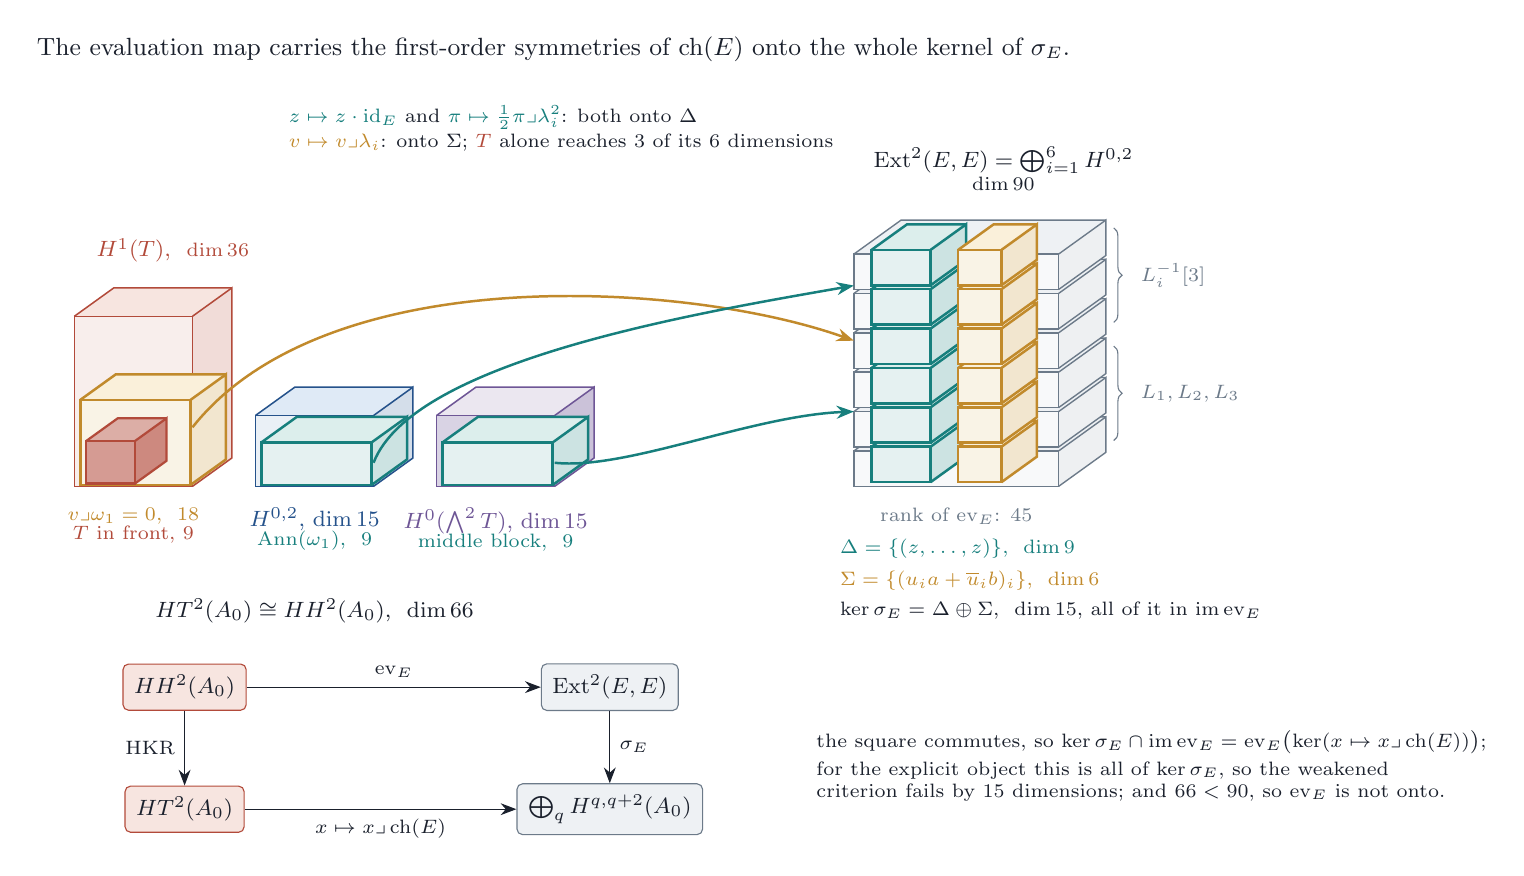
\begin{tikzpicture}[font=\small,text=PInk]

\node[anchor=west,font=\small,text=PInk] at (-0.6,5.55)
  {The evaluation map carries the first-order symmetries of $\ch(E)$ onto the whole kernel of $\sigma_{E}$.};

%% =====================================================================
%% Left: HT^2 as three slabs, heights 36 : 15 : 15 (scale 0.06 per dim)
%% =====================================================================
% H^1(T), height 2.16; the 18 killing omega_1 as the lower part, T (9) in front
\slab{0}{0}{0}{1.5}{1.0}{2.16}{vv}
\slab{0.05}{0.05}{0}{1.4}{0.9}{1.08}{sig}
\slab{0.10}{0.10}{0}{0.62}{0.8}{0.54}{tt}
% H^{0,2}, height 0.9; the annihilator (9) as the lower part
\slab{2.3}{0}{0}{1.5}{1.0}{0.9}{zz}
\slab{2.35}{0.05}{0}{1.4}{0.9}{0.54}{ker}
% wedge^2 T, height 0.9; the middle block (9) as the lower part
\slab{4.6}{0}{0}{1.5}{1.0}{0.9}{pp}
\slab{4.65}{0.05}{0}{1.4}{0.9}{0.54}{ker}

\begin{scope}[obl]
  \coordinate (Vt) at (0.75,1.0,2.16);
  \coordinate (Zt) at (3.05,1.0,0.9);
  \coordinate (Pt) at (5.35,1.0,0.9);
  \coordinate (Vk) at (1.5,0.0,0.75);
  \coordinate (Zk) at (3.8,0.0,0.30);
  \coordinate (Pk) at (6.1,0.0,0.30);
  \coordinate (Vb) at (0.75,0,0);
  \coordinate (Zb) at (3.05,0,0);
  \coordinate (Pb) at (5.35,0,0);
\end{scope}
\node[anchor=south,align=center,font=\footnotesize,text=PClay] at ([yshift=2mm]Vt)
  {$H^{1}(T)$, \ {\scriptsize $\dim 36$}};
\node[anchor=north,align=center,font=\scriptsize,text=POchre] at ([yshift=-1.5mm]Vb)
  {$v\lrcorner\omega_{1}=0$, \ $18$\\[-1pt]{\color{PClay}$T$ in front, $9$}};
\node[anchor=north,align=center,font=\scriptsize,text=PTeal] at ([yshift=-1.5mm]Zb)
  {{\color{PBlue}\footnotesize $H^{0,2}$, $\dim 15$}\\[-1pt]$\operatorname{Ann}(\omega_{1})$, \ $9$};
\node[anchor=north,align=center,font=\scriptsize,text=PTeal] at ([yshift=-1.5mm]Pb)
  {{\color{PViolet}\footnotesize $H^{0}(\bigwedge^{2}T)$, $\dim 15$}\\[-1pt]middle block, \ $9$};
\node[anchor=north,font=\footnotesize,text=PInk] at (3.05,-1.3)
  {$HT^{2}(A_{0})\cong HH^{2}(A_{0})$, \ $\dim 66$};

%% =====================================================================
%% Right: Ext^2(E,E) as six stacked copies of H^{0,2}, height 0.45 each
%% =====================================================================
\begin{scope}[shift={(9.9,0)}]
  \foreach \k in {0,...,5} {
    \pgfmathsetmacro{\zz}{0.5*\k}
    \slab{0}{0}{\zz}{2.6}{1.2}{0.45}{ext}
  }
  \foreach \k in {0,...,5} {
    \pgfmathsetmacro{\zz}{0.5*\k}
    \slab{0.15}{0.15}{\zz}{0.75}{0.9}{0.45}{ker}
  }
  \foreach \k in {0,...,5} {
    \pgfmathsetmacro{\zz}{0.5*\k}
    \slab{1.25}{0.15}{\zz}{0.55}{0.9}{0.45}{sig}
  }
  \begin{scope}[obl]
    \coordinate (Et) at (1.3,1.2,3.0);
    \coordinate (Eb) at (1.3,0,0);
    \coordinate (Rlo) at (2.6,1.2,0.15);
    \coordinate (Rmid) at (2.6,1.2,1.35);
    \coordinate (Rmid2) at (2.6,1.2,1.65);
    \coordinate (Rhi) at (2.6,1.2,2.85);
  \end{scope}
  \node[anchor=south,align=center,font=\footnotesize,text=PInk] at ([yshift=2mm]Et)
    {$\operatorname{Ext}^{2}(E,E)=\bigoplus_{i=1}^{6}H^{0,2}$\\[-1pt]{\scriptsize $\dim 90$}};
  \node[anchor=north,align=center,font=\scriptsize,text=PSlate] at ([yshift=-1.5mm]Eb)
    {rank of $\operatorname{ev}_{E}$: $45$};
  \draw[decorate,decoration={brace,amplitude=3pt},PSlate] ([xshift=1mm]Rmid) -- ([xshift=1mm]Rlo)
    node[midway,xshift=2.2mm,anchor=west,font=\scriptsize,text=PSlate] {$L_{1},L_{2},L_{3}$};
  \draw[decorate,decoration={brace,amplitude=3pt},PSlate] ([xshift=1mm]Rhi) -- ([xshift=1mm]Rmid2)
    node[midway,xshift=2.2mm,anchor=west,font=\scriptsize,text=PSlate] {$L_{i}^{-1}[3]$};
\end{scope}

% the two parts of the kernel, described below the stack
\node[anchor=north west,align=left,font=\scriptsize,text=PTeal] at (9.6,-0.55)
  {$\Delta=\{(z,\dots,z)\}$, \ $\dim 9$};
\node[anchor=north west,align=left,font=\scriptsize,text=POchre] at (9.6,-0.95)
  {$\Sigma=\{(u_{i}a+\bbar u_{i}b)_{i}\}$, \ $\dim 6$};
\node[anchor=north west,align=left,font=\scriptsize,text=PInk] at (9.6,-1.35)
  {$\ker\sigma_{E}=\Delta\oplus\Sigma$, \ $\dim 15$, all of it in $\operatorname{im}\operatorname{ev}_{E}$};

%% =====================================================================
%% The evaluation arrows on the three kernels, routed above the slabs
%% =====================================================================
\draw[POchre,line width=0.9pt,-{Stealth[length=2.2mm]}]
  (Vk) .. controls (3.2,2.9) and (7.8,2.6) .. (9.9,1.85);
\draw[PTeal,line width=0.9pt,-{Stealth[length=2.2mm]}]
  (Zk) .. controls (4.3,1.6) and (7.9,2.2) .. (9.9,2.55);
\draw[PTeal,line width=0.9pt,-{Stealth[length=2.2mm]}]
  (Pk) .. controls (7.0,0.2) and (8.6,0.9) .. (9.9,0.95);

\node[anchor=west,align=left,font=\scriptsize,text=PInk] at (2.6,4.55)
  {{\color{PTeal}$z\mapsto z\cdot\mathrm{id}_{E}$} and
   {\color{PTeal}$\pi\mapsto\tfrac12\pi\lrcorner\lambda_{i}^{2}$}: both onto $\Delta$\\[1pt]
   {\color{POchre}$v\mapsto v\lrcorner\lambda_{i}$}: onto $\Sigma$;
   {\color{PClay}$T$} alone reaches $3$ of its $6$ dimensions};

%% =====================================================================
%% Below: the commutative square
%% =====================================================================
\begin{scope}[shift={(0,-2.55)}]
  \node[draw=PClay,fill=WClay,rounded corners=2pt,inner sep=4pt,font=\footnotesize] (HH) at (1.4,0) {$HH^{2}(A_{0})$};
  \node[draw=PSlate,fill=WSlate,rounded corners=2pt,inner sep=4pt,font=\footnotesize] (EX) at (6.8,0) {$\operatorname{Ext}^{2}(E,E)$};
  \node[draw=PClay,fill=WClay,rounded corners=2pt,inner sep=4pt,font=\footnotesize] (HT) at (1.4,-1.55) {$HT^{2}(A_{0})$};
  \node[draw=PSlate,fill=WSlate,rounded corners=2pt,inner sep=4pt,font=\footnotesize] (HQ) at (6.8,-1.55) {$\bigoplus_{q}H^{q,q+2}(A_{0})$};
  \draw[PInk,-{Stealth[length=2mm]}] (HH) -- node[above,font=\scriptsize] {$\operatorname{ev}_{E}$} (EX);
  \draw[PInk,-{Stealth[length=2mm]}] (HH) -- node[left,font=\scriptsize] {HKR} (HT);
  \draw[PInk,-{Stealth[length=2mm]}] (EX) -- node[right,font=\scriptsize] {$\sigma_{E}$} (HQ);
  \draw[PInk,-{Stealth[length=2mm]}] (HT) -- node[below,font=\scriptsize] {$x\mapsto x\lrcorner\ch(E)$} (HQ);
\end{scope}
\node[anchor=west,align=left,font=\scriptsize,text=PInk] at (9.3,-3.55)
  {the square commutes, so
   $\ker\sigma_{E}\cap\operatorname{im}\operatorname{ev}_{E}
     =\operatorname{ev}_{E}\bigl(\ker(x\mapsto x\lrcorner\ch(E))\bigr)$;\\[2pt]
   for the explicit object this is all of $\ker\sigma_{E}$, so the weakened\\
   criterion fails by $15$ dimensions; and $66<90$, so $\operatorname{ev}_{E}$ is not onto.};

\end{tikzpicture}
\end{document}
